\documentclass[]{article}
\usepackage{lmodern}
\usepackage{amssymb,amsmath}
\usepackage{ifxetex,ifluatex}
\usepackage{fixltx2e} % provides \textsubscript
\ifnum 0\ifxetex 1\fi\ifluatex 1\fi=0 % if pdftex
  \usepackage[T1]{fontenc}
  \usepackage[utf8]{inputenc}
\else % if luatex or xelatex
  \ifxetex
    \usepackage{mathspec}
  \else
    \usepackage{fontspec}
  \fi
  \defaultfontfeatures{Ligatures=TeX,Scale=MatchLowercase}
\fi
% use upquote if available, for straight quotes in verbatim environments
\IfFileExists{upquote.sty}{\usepackage{upquote}}{}
% use microtype if available
\IfFileExists{microtype.sty}{%
\usepackage{microtype}
\UseMicrotypeSet[protrusion]{basicmath} % disable protrusion for tt fonts
}{}
\usepackage[margin=1in]{geometry}
\usepackage{hyperref}
\hypersetup{unicode=true,
            pdftitle={Breast Cancer Detection},
            pdfborder={0 0 0},
            breaklinks=true}
\urlstyle{same}  % don't use monospace font for urls
\usepackage{color}
\usepackage{fancyvrb}
\newcommand{\VerbBar}{|}
\newcommand{\VERB}{\Verb[commandchars=\\\{\}]}
\DefineVerbatimEnvironment{Highlighting}{Verbatim}{commandchars=\\\{\}}
% Add ',fontsize=\small' for more characters per line
\usepackage{framed}
\definecolor{shadecolor}{RGB}{248,248,248}
\newenvironment{Shaded}{\begin{snugshade}}{\end{snugshade}}
\newcommand{\AlertTok}[1]{\textcolor[rgb]{0.94,0.16,0.16}{#1}}
\newcommand{\AnnotationTok}[1]{\textcolor[rgb]{0.56,0.35,0.01}{\textbf{\textit{#1}}}}
\newcommand{\AttributeTok}[1]{\textcolor[rgb]{0.77,0.63,0.00}{#1}}
\newcommand{\BaseNTok}[1]{\textcolor[rgb]{0.00,0.00,0.81}{#1}}
\newcommand{\BuiltInTok}[1]{#1}
\newcommand{\CharTok}[1]{\textcolor[rgb]{0.31,0.60,0.02}{#1}}
\newcommand{\CommentTok}[1]{\textcolor[rgb]{0.56,0.35,0.01}{\textit{#1}}}
\newcommand{\CommentVarTok}[1]{\textcolor[rgb]{0.56,0.35,0.01}{\textbf{\textit{#1}}}}
\newcommand{\ConstantTok}[1]{\textcolor[rgb]{0.00,0.00,0.00}{#1}}
\newcommand{\ControlFlowTok}[1]{\textcolor[rgb]{0.13,0.29,0.53}{\textbf{#1}}}
\newcommand{\DataTypeTok}[1]{\textcolor[rgb]{0.13,0.29,0.53}{#1}}
\newcommand{\DecValTok}[1]{\textcolor[rgb]{0.00,0.00,0.81}{#1}}
\newcommand{\DocumentationTok}[1]{\textcolor[rgb]{0.56,0.35,0.01}{\textbf{\textit{#1}}}}
\newcommand{\ErrorTok}[1]{\textcolor[rgb]{0.64,0.00,0.00}{\textbf{#1}}}
\newcommand{\ExtensionTok}[1]{#1}
\newcommand{\FloatTok}[1]{\textcolor[rgb]{0.00,0.00,0.81}{#1}}
\newcommand{\FunctionTok}[1]{\textcolor[rgb]{0.00,0.00,0.00}{#1}}
\newcommand{\ImportTok}[1]{#1}
\newcommand{\InformationTok}[1]{\textcolor[rgb]{0.56,0.35,0.01}{\textbf{\textit{#1}}}}
\newcommand{\KeywordTok}[1]{\textcolor[rgb]{0.13,0.29,0.53}{\textbf{#1}}}
\newcommand{\NormalTok}[1]{#1}
\newcommand{\OperatorTok}[1]{\textcolor[rgb]{0.81,0.36,0.00}{\textbf{#1}}}
\newcommand{\OtherTok}[1]{\textcolor[rgb]{0.56,0.35,0.01}{#1}}
\newcommand{\PreprocessorTok}[1]{\textcolor[rgb]{0.56,0.35,0.01}{\textit{#1}}}
\newcommand{\RegionMarkerTok}[1]{#1}
\newcommand{\SpecialCharTok}[1]{\textcolor[rgb]{0.00,0.00,0.00}{#1}}
\newcommand{\SpecialStringTok}[1]{\textcolor[rgb]{0.31,0.60,0.02}{#1}}
\newcommand{\StringTok}[1]{\textcolor[rgb]{0.31,0.60,0.02}{#1}}
\newcommand{\VariableTok}[1]{\textcolor[rgb]{0.00,0.00,0.00}{#1}}
\newcommand{\VerbatimStringTok}[1]{\textcolor[rgb]{0.31,0.60,0.02}{#1}}
\newcommand{\WarningTok}[1]{\textcolor[rgb]{0.56,0.35,0.01}{\textbf{\textit{#1}}}}
\usepackage{graphicx,grffile}
\makeatletter
\def\maxwidth{\ifdim\Gin@nat@width>\linewidth\linewidth\else\Gin@nat@width\fi}
\def\maxheight{\ifdim\Gin@nat@height>\textheight\textheight\else\Gin@nat@height\fi}
\makeatother
% Scale images if necessary, so that they will not overflow the page
% margins by default, and it is still possible to overwrite the defaults
% using explicit options in \includegraphics[width, height, ...]{}
\setkeys{Gin}{width=\maxwidth,height=\maxheight,keepaspectratio}
\IfFileExists{parskip.sty}{%
\usepackage{parskip}
}{% else
\setlength{\parindent}{0pt}
\setlength{\parskip}{6pt plus 2pt minus 1pt}
}
\setlength{\emergencystretch}{3em}  % prevent overfull lines
\providecommand{\tightlist}{%
  \setlength{\itemsep}{0pt}\setlength{\parskip}{0pt}}
\setcounter{secnumdepth}{0}
% Redefines (sub)paragraphs to behave more like sections
\ifx\paragraph\undefined\else
\let\oldparagraph\paragraph
\renewcommand{\paragraph}[1]{\oldparagraph{#1}\mbox{}}
\fi
\ifx\subparagraph\undefined\else
\let\oldsubparagraph\subparagraph
\renewcommand{\subparagraph}[1]{\oldsubparagraph{#1}\mbox{}}
\fi

%%% Use protect on footnotes to avoid problems with footnotes in titles
\let\rmarkdownfootnote\footnote%
\def\footnote{\protect\rmarkdownfootnote}

%%% Change title format to be more compact
\usepackage{titling}

% Create subtitle command for use in maketitle
\providecommand{\subtitle}[1]{
  \posttitle{
    \begin{center}\large#1\end{center}
    }
}

\setlength{\droptitle}{-2em}

  \title{Breast Cancer Detection}
    \pretitle{\vspace{\droptitle}\centering\huge}
  \posttitle{\par}
    \author{}
    \preauthor{}\postauthor{}
    \date{}
    \predate{}\postdate{}
  

\begin{document}
\maketitle

Early detection of breast cancer is crucial for successful treatment.
Conventional methods such as breast biopsy are more invasive and must be
performed by a human specialist, which would be time consuming and not
scalable. However, samples obtained with less invasive techniques like
fine needle aspiration can be easily digitized and used for
computer-aided diagnosis. To this end, the use of machine learning
methods can significantly reduce the cost and time for the diagnostic
process. This code snippet shows the reader how to train a Naive Bayes
(NB) classifier for breast cancer detection.

\textbf{The dataset:} We utilise the dataset available at
\url{http://archive.ics.uci.edu/ml/datasets/breast+cancer+wisconsin+\%28diagnostic\%29}

\textbf{Machine learning (ML) task:} Given a feature set we need to
clasify a tumor as benign or malignant. So, our ML task in this problem
would be a classification. Let's explore the dataset.

\begin{Shaded}
\begin{Highlighting}[]
\NormalTok{myData <-}\StringTok{ }\KeywordTok{read.csv}\NormalTok{(}\StringTok{"CancerData.csv"}\NormalTok{, }\DataTypeTok{header=}\NormalTok{T)}
\KeywordTok{dim}\NormalTok{(myData) }\CommentTok{# check dimensions of myData}
\end{Highlighting}
\end{Shaded}

\begin{verbatim}
## [1] 569  32
\end{verbatim}

\begin{Shaded}
\begin{Highlighting}[]
\KeywordTok{sapply}\NormalTok{(myData, class) }\CommentTok{# check the data types of each feature}
\end{Highlighting}
\end{Shaded}

\begin{verbatim}
##                   id                label          radius.mean 
##            "integer"             "factor"            "numeric" 
##       perimeter.mean            area.mean      smoothness.mean 
##            "numeric"            "numeric"            "numeric" 
##     compactness.mean       concavity.mean         concave.mean 
##            "numeric"            "numeric"            "numeric" 
##        symmetry.mean         fractal.mean     perimeter.mean.1 
##            "numeric"            "numeric"            "numeric" 
##      radius.stderror   perimeter.stderror        area.stderror 
##            "numeric"            "numeric"            "numeric" 
##  smoothness.stderror compactness.stderror   concavity.stderror 
##            "numeric"            "numeric"            "numeric" 
##     concave.stderror    symmetry.stderror     fractal.stderror 
##            "numeric"            "numeric"            "numeric" 
## perimeter.stderror.1         radius.worst      perimeter.worst 
##            "numeric"            "numeric"            "numeric" 
##           area.worst     smoothness.worst    compactness.worst 
##            "numeric"            "numeric"            "numeric" 
##      concavity.worst        concave.worst       symmetry.worst 
##            "numeric"            "numeric"            "numeric" 
##        fractal.worst    perimeter.worst.1 
##            "numeric"            "numeric"
\end{verbatim}

\begin{Shaded}
\begin{Highlighting}[]
\KeywordTok{levels}\NormalTok{(myData}\OperatorTok{$}\NormalTok{label) }\CommentTok{# check different levels (values) for each class}
\end{Highlighting}
\end{Shaded}

\begin{verbatim}
## [1] "B" "M"
\end{verbatim}

\begin{Shaded}
\begin{Highlighting}[]
\KeywordTok{head}\NormalTok{(myData) }\CommentTok{# have a look at top data points in myData}
\end{Highlighting}
\end{Shaded}

\begin{verbatim}
##         id label radius.mean perimeter.mean area.mean smoothness.mean
## 1   842302     M       17.99          10.38    122.80          1001.0
## 2   842517     M       20.57          17.77    132.90          1326.0
## 3 84300903     M       19.69          21.25    130.00          1203.0
## 4 84348301     M       11.42          20.38     77.58           386.1
## 5 84358402     M       20.29          14.34    135.10          1297.0
## 6   843786     M       12.45          15.70     82.57           477.1
##   compactness.mean concavity.mean concave.mean symmetry.mean fractal.mean
## 1          0.11840        0.27760       0.3001       0.14710       0.2419
## 2          0.08474        0.07864       0.0869       0.07017       0.1812
## 3          0.10960        0.15990       0.1974       0.12790       0.2069
## 4          0.14250        0.28390       0.2414       0.10520       0.2597
## 5          0.10030        0.13280       0.1980       0.10430       0.1809
## 6          0.12780        0.17000       0.1578       0.08089       0.2087
##   perimeter.mean.1 radius.stderror perimeter.stderror area.stderror
## 1          0.07871          1.0950             0.9053         8.589
## 2          0.05667          0.5435             0.7339         3.398
## 3          0.05999          0.7456             0.7869         4.585
## 4          0.09744          0.4956             1.1560         3.445
## 5          0.05883          0.7572             0.7813         5.438
## 6          0.07613          0.3345             0.8902         2.217
##   smoothness.stderror compactness.stderror concavity.stderror
## 1              153.40             0.006399            0.04904
## 2               74.08             0.005225            0.01308
## 3               94.03             0.006150            0.04006
## 4               27.23             0.009110            0.07458
## 5               94.44             0.011490            0.02461
## 6               27.19             0.007510            0.03345
##   concave.stderror symmetry.stderror fractal.stderror perimeter.stderror.1
## 1          0.05373           0.01587          0.03003             0.006193
## 2          0.01860           0.01340          0.01389             0.003532
## 3          0.03832           0.02058          0.02250             0.004571
## 4          0.05661           0.01867          0.05963             0.009208
## 5          0.05688           0.01885          0.01756             0.005115
## 6          0.03672           0.01137          0.02165             0.005082
##   radius.worst perimeter.worst area.worst smoothness.worst
## 1        25.38           17.33     184.60           2019.0
## 2        24.99           23.41     158.80           1956.0
## 3        23.57           25.53     152.50           1709.0
## 4        14.91           26.50      98.87            567.7
## 5        22.54           16.67     152.20           1575.0
## 6        15.47           23.75     103.40            741.6
##   compactness.worst concavity.worst concave.worst symmetry.worst
## 1            0.1622          0.6656        0.7119         0.2654
## 2            0.1238          0.1866        0.2416         0.1860
## 3            0.1444          0.4245        0.4504         0.2430
## 4            0.2098          0.8663        0.6869         0.2575
## 5            0.1374          0.2050        0.4000         0.1625
## 6            0.1791          0.5249        0.5355         0.1741
##   fractal.worst perimeter.worst.1
## 1        0.4601           0.11890
## 2        0.2750           0.08902
## 3        0.3613           0.08758
## 4        0.6638           0.17300
## 5        0.2364           0.07678
## 6        0.3985           0.12440
\end{verbatim}

\begin{Shaded}
\begin{Highlighting}[]
\KeywordTok{summary}\NormalTok{(myData) }\CommentTok{# a summary of class distributions}
\end{Highlighting}
\end{Shaded}

\begin{verbatim}
##        id            label    radius.mean     perimeter.mean 
##  Min.   :     8670   B:357   Min.   : 6.981   Min.   : 9.71  
##  1st Qu.:   869218   M:212   1st Qu.:11.700   1st Qu.:16.17  
##  Median :   906024           Median :13.370   Median :18.84  
##  Mean   : 30371831           Mean   :14.127   Mean   :19.29  
##  3rd Qu.:  8813129           3rd Qu.:15.780   3rd Qu.:21.80  
##  Max.   :911320502           Max.   :28.110   Max.   :39.28  
##    area.mean      smoothness.mean  compactness.mean  concavity.mean   
##  Min.   : 43.79   Min.   : 143.5   Min.   :0.05263   Min.   :0.01938  
##  1st Qu.: 75.17   1st Qu.: 420.3   1st Qu.:0.08637   1st Qu.:0.06492  
##  Median : 86.24   Median : 551.1   Median :0.09587   Median :0.09263  
##  Mean   : 91.97   Mean   : 654.9   Mean   :0.09636   Mean   :0.10434  
##  3rd Qu.:104.10   3rd Qu.: 782.7   3rd Qu.:0.10530   3rd Qu.:0.13040  
##  Max.   :188.50   Max.   :2501.0   Max.   :0.16340   Max.   :0.34540  
##   concave.mean     symmetry.mean      fractal.mean    perimeter.mean.1 
##  Min.   :0.00000   Min.   :0.00000   Min.   :0.1060   Min.   :0.04996  
##  1st Qu.:0.02956   1st Qu.:0.02031   1st Qu.:0.1619   1st Qu.:0.05770  
##  Median :0.06154   Median :0.03350   Median :0.1792   Median :0.06154  
##  Mean   :0.08880   Mean   :0.04892   Mean   :0.1812   Mean   :0.06280  
##  3rd Qu.:0.13070   3rd Qu.:0.07400   3rd Qu.:0.1957   3rd Qu.:0.06612  
##  Max.   :0.42680   Max.   :0.20120   Max.   :0.3040   Max.   :0.09744  
##  radius.stderror  perimeter.stderror area.stderror    smoothness.stderror
##  Min.   :0.1115   Min.   :0.3602     Min.   : 0.757   Min.   :  6.802    
##  1st Qu.:0.2324   1st Qu.:0.8339     1st Qu.: 1.606   1st Qu.: 17.850    
##  Median :0.3242   Median :1.1080     Median : 2.287   Median : 24.530    
##  Mean   :0.4052   Mean   :1.2169     Mean   : 2.866   Mean   : 40.337    
##  3rd Qu.:0.4789   3rd Qu.:1.4740     3rd Qu.: 3.357   3rd Qu.: 45.190    
##  Max.   :2.8730   Max.   :4.8850     Max.   :21.980   Max.   :542.200    
##  compactness.stderror concavity.stderror concave.stderror 
##  Min.   :0.001713     Min.   :0.002252   Min.   :0.00000  
##  1st Qu.:0.005169     1st Qu.:0.013080   1st Qu.:0.01509  
##  Median :0.006380     Median :0.020450   Median :0.02589  
##  Mean   :0.007041     Mean   :0.025478   Mean   :0.03189  
##  3rd Qu.:0.008146     3rd Qu.:0.032450   3rd Qu.:0.04205  
##  Max.   :0.031130     Max.   :0.135400   Max.   :0.39600  
##  symmetry.stderror  fractal.stderror   perimeter.stderror.1
##  Min.   :0.000000   Min.   :0.007882   Min.   :0.0008948   
##  1st Qu.:0.007638   1st Qu.:0.015160   1st Qu.:0.0022480   
##  Median :0.010930   Median :0.018730   Median :0.0031870   
##  Mean   :0.011796   Mean   :0.020542   Mean   :0.0037949   
##  3rd Qu.:0.014710   3rd Qu.:0.023480   3rd Qu.:0.0045580   
##  Max.   :0.052790   Max.   :0.078950   Max.   :0.0298400   
##   radius.worst   perimeter.worst   area.worst     smoothness.worst
##  Min.   : 7.93   Min.   :12.02   Min.   : 50.41   Min.   : 185.2  
##  1st Qu.:13.01   1st Qu.:21.08   1st Qu.: 84.11   1st Qu.: 515.3  
##  Median :14.97   Median :25.41   Median : 97.66   Median : 686.5  
##  Mean   :16.27   Mean   :25.68   Mean   :107.26   Mean   : 880.6  
##  3rd Qu.:18.79   3rd Qu.:29.72   3rd Qu.:125.40   3rd Qu.:1084.0  
##  Max.   :36.04   Max.   :49.54   Max.   :251.20   Max.   :4254.0  
##  compactness.worst concavity.worst   concave.worst    symmetry.worst   
##  Min.   :0.07117   Min.   :0.02729   Min.   :0.0000   Min.   :0.00000  
##  1st Qu.:0.11660   1st Qu.:0.14720   1st Qu.:0.1145   1st Qu.:0.06493  
##  Median :0.13130   Median :0.21190   Median :0.2267   Median :0.09993  
##  Mean   :0.13237   Mean   :0.25427   Mean   :0.2722   Mean   :0.11461  
##  3rd Qu.:0.14600   3rd Qu.:0.33910   3rd Qu.:0.3829   3rd Qu.:0.16140  
##  Max.   :0.22260   Max.   :1.05800   Max.   :1.2520   Max.   :0.29100  
##  fractal.worst    perimeter.worst.1
##  Min.   :0.1565   Min.   :0.05504  
##  1st Qu.:0.2504   1st Qu.:0.07146  
##  Median :0.2822   Median :0.08004  
##  Mean   :0.2901   Mean   :0.08395  
##  3rd Qu.:0.3179   3rd Qu.:0.09208  
##  Max.   :0.6638   Max.   :0.20750
\end{verbatim}

\begin{Shaded}
\begin{Highlighting}[]
\KeywordTok{prop.table}\NormalTok{(}\KeywordTok{table}\NormalTok{(myData}\OperatorTok{$}\NormalTok{label)) }\CommentTok{# Ratio between two classes}
\end{Highlighting}
\end{Shaded}

\begin{verbatim}
## 
##         B         M 
## 0.6274165 0.3725835
\end{verbatim}

\begin{Shaded}
\begin{Highlighting}[]
\KeywordTok{library}\NormalTok{(corrplot) }\CommentTok{# Load libraries to plot correlation}
\KeywordTok{library}\NormalTok{(RColorBrewer)}
\NormalTok{M <-}\KeywordTok{cor}\NormalTok{(myData[,}\DecValTok{3}\OperatorTok{:}\KeywordTok{ncol}\NormalTok{(myData)])}
\KeywordTok{corrplot}\NormalTok{(M, }\DataTypeTok{type=}\StringTok{"upper"}\NormalTok{, }\DataTypeTok{order=}\StringTok{"hclust"}\NormalTok{, }\DataTypeTok{col=}\KeywordTok{brewer.pal}\NormalTok{(}\DataTypeTok{n=}\DecValTok{10}\NormalTok{, }\DataTypeTok{name=}\StringTok{"RdYlBu"}\NormalTok{))}
\end{Highlighting}
\end{Shaded}

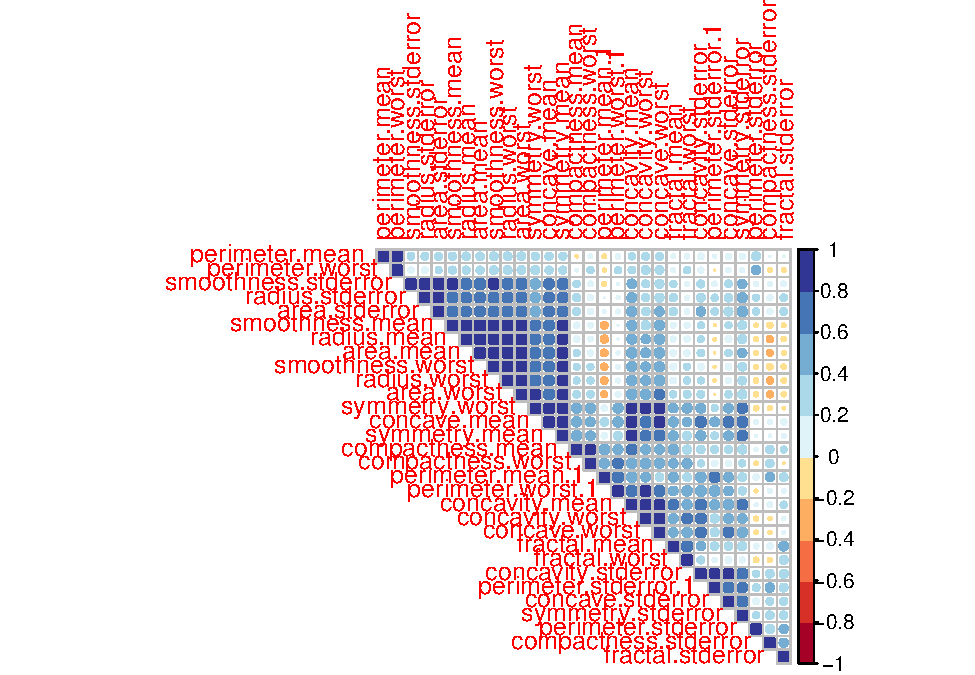
\includegraphics{Breast-cancer_files/figure-latex/unnamed-chunk-1-1.pdf}

We notice that the data is slightly imbalanced and there are highly
correlated features. However, we do not remove correlated features from
the dataset nor deal with the class imbalanced problem in this analysis
as the purpose of this post to demonstrate you how to train NB model for
the dataset. Therefore we will use our dataset as it's in model
building.

\textbf{Creating training and validation datasets:} We're going to
follow the convention of 80/20 samples ratio to partition the dataset as
was in the previous example. We use the createDataPartition function
from the caret package for this purpose.

\begin{Shaded}
\begin{Highlighting}[]
\KeywordTok{set.seed}\NormalTok{(}\DecValTok{12}\NormalTok{)}
\CommentTok{#install.packages("caret") #If the caret package is not installed on your system, uncomment this line to install it first}
\KeywordTok{library}\NormalTok{(caret) }\CommentTok{#Loading the library}
\NormalTok{tr_index <-}\StringTok{ }\KeywordTok{createDataPartition}\NormalTok{(myData}\OperatorTok{$}\NormalTok{label, }\DataTypeTok{p=}\FloatTok{0.80}\NormalTok{, }\DataTypeTok{list=}\OtherTok{FALSE}\NormalTok{) }\CommentTok{# List of 80% of the rows}
\NormalTok{trainSet <-}\StringTok{ }\NormalTok{myData[tr_index,] }\CommentTok{# select 80% of the data for the trainSet}
\NormalTok{testSet <-}\StringTok{ }\NormalTok{myData[}\OperatorTok{-}\NormalTok{tr_index,] }\CommentTok{# Select the remaining 20% of data for testSet}
\end{Highlighting}
\end{Shaded}

\textbf{Building a NB classifier:} Now we will train our NB classifier
using the above trainSet. For this purpose, we will utilize e1071
package in R.

\begin{Shaded}
\begin{Highlighting}[]
\CommentTok{#install.packages("e1071") #If the e1071 package is not installed on your system, uncomment this line to install it first}
\KeywordTok{library}\NormalTok{(e1071)}
\NormalTok{NBclassfier=}\KeywordTok{naiveBayes}\NormalTok{(label}\OperatorTok{~}\NormalTok{., }\DataTypeTok{data=}\NormalTok{trainSet[,}\DecValTok{2}\OperatorTok{:}\KeywordTok{ncol}\NormalTok{(trainSet)]) }\CommentTok{# Once you call this line, R fits the NB model using trainSet}
\KeywordTok{print}\NormalTok{(NBclassfier) }\CommentTok{# Check the newly fitted model to see if everything is OK.}
\end{Highlighting}
\end{Shaded}

\begin{verbatim}
## 
## Naive Bayes Classifier for Discrete Predictors
## 
## Call:
## naiveBayes.default(x = X, y = Y, laplace = laplace)
## 
## A-priori probabilities:
## Y
##        B        M 
## 0.627193 0.372807 
## 
## Conditional probabilities:
##    radius.mean
## Y       [,1]     [,2]
##   B 12.28738 1.730600
##   M 17.51965 3.101673
## 
##    perimeter.mean
## Y       [,1]    [,2]
##   B 17.69794 4.01135
##   M 21.70582 3.67748
## 
##    area.mean
## Y        [,1]     [,2]
##   B  79.04063 11.47299
##   M 115.71647 21.11783
## 
##    smoothness.mean
## Y       [,1]     [,2]
##   B 472.8682 131.9559
##   M 981.2335 350.8699
## 
##    compactness.mean
## Y         [,1]       [,2]
##   B 0.09269678 0.01338821
##   M 0.10214365 0.01246641
## 
##    concavity.mean
## Y         [,1]       [,2]
##   B 0.08142664 0.03404852
##   M 0.14466382 0.05492977
## 
##    concave.mean
## Y         [,1]       [,2]
##   B 0.04696074 0.04243983
##   M 0.15944900 0.07307398
## 
##    symmetry.mean
## Y         [,1]       [,2]
##   B 0.02639213 0.01590501
##   M 0.08736982 0.03391047
## 
##    fractal.mean
## Y        [,1]       [,2]
##   B 0.1739182 0.02549547
##   M 0.1923547 0.02667948
## 
##    perimeter.mean.1
## Y         [,1]        [,2]
##   B 0.06271584 0.006633772
##   M 0.06238747 0.007568478
## 
##    radius.stderror
## Y        [,1]      [,2]
##   B 0.2863584 0.1094833
##   M 0.5917812 0.3223556
## 
##    perimeter.stderror
## Y       [,1]      [,2]
##   B 1.203570 0.5954131
##   M 1.228599 0.5126423
## 
##    area.stderror
## Y       [,1]      [,2]
##   B 2.032098 0.7884899
##   M 4.221765 2.4232362
## 
##    smoothness.stderror
## Y       [,1]      [,2]
##   B 21.52602  8.606888
##   M 69.64241 53.285735
## 
##    compactness.stderror
## Y          [,1]        [,2]
##   B 0.007089241 0.003092158
##   M 0.006748429 0.003056157
## 
##    concavity.stderror
## Y         [,1]       [,2]
##   B 0.02166044 0.01556083
##   M 0.03254798 0.01898363
## 
##    concave.stderror
## Y         [,1]       [,2]
##   B 0.02611506 0.03095271
##   M 0.04198171 0.02209141
## 
##    symmetry.stderror
## Y          [,1]        [,2]
##   B 0.009995203 0.005592443
##   M 0.015085406 0.005619178
## 
##    fractal.stderror
## Y         [,1]        [,2]
##   B 0.02048688 0.006980606
##   M 0.02064860 0.010134221
## 
##    perimeter.stderror.1
## Y          [,1]        [,2]
##   B 0.003579784 0.002721344
##   M 0.004118147 0.002122180
## 
##    radius.worst
## Y       [,1]     [,2]
##   B 13.53490 1.953745
##   M 21.05824 4.019718
## 
##    perimeter.worst
## Y       [,1]     [,2]
##   B 23.18003 5.503008
##   M 29.42494 5.245644
## 
##    area.worst
## Y        [,1]     [,2]
##   B  88.15136 13.37712
##   M 140.86300 27.51031
## 
##    smoothness.worst
## Y        [,1]     [,2]
##   B  571.4441 163.0309
##   M 1403.1141 540.0212
## 
##    compactness.worst
## Y        [,1]       [,2]
##   B 0.1246396 0.02006242
##   M 0.1438341 0.02225645
## 
##    concavity.worst
## Y        [,1]       [,2]
##   B 0.1867495 0.09394689
##   M 0.3753983 0.17589729
## 
##    concave.worst
## Y        [,1]      [,2]
##   B 0.1680108 0.1316073
##   M 0.4500905 0.1837993
## 
##    symmetry.worst
## Y         [,1]       [,2]
##   B 0.07582791 0.03488616
##   M 0.18157918 0.04636119
## 
##    fractal.worst
## Y        [,1]       [,2]
##   B 0.2692129 0.04188110
##   M 0.3242171 0.07665267
## 
##    perimeter.worst.1
## Y         [,1]       [,2]
##   B 0.07930696 0.01386718
##   M 0.09153382 0.02181732
\end{verbatim}

\textbf{Make predictions:} Now let's apply the above model to assign
labels for test cases in testSet. Then we create the confusion matrix, a
table that is often used to describe the performance of a classifier.

\begin{Shaded}
\begin{Highlighting}[]
\NormalTok{  testPrediction=}\KeywordTok{predict}\NormalTok{(NBclassfier, }\DataTypeTok{newdata=}\NormalTok{testSet[,}\DecValTok{2}\OperatorTok{:}\KeywordTok{ncol}\NormalTok{(testSet)], }\DataTypeTok{type=}\StringTok{"class"}\NormalTok{) }\CommentTok{# Assign labels for each test case}
  \KeywordTok{confusionMatrix}\NormalTok{(testPrediction, testSet}\OperatorTok{$}\NormalTok{label, }\DataTypeTok{positive =} \StringTok{"M"}\NormalTok{) }\CommentTok{# Print confusion matrix }
\end{Highlighting}
\end{Shaded}

\begin{verbatim}
## Confusion Matrix and Statistics
## 
##           Reference
## Prediction  B  M
##          B 68  4
##          M  3 38
##                                           
##                Accuracy : 0.9381          
##                  95% CI : (0.8765, 0.9747)
##     No Information Rate : 0.6283          
##     P-Value [Acc > NIR] : 1.718e-14       
##                                           
##                   Kappa : 0.8667          
##                                           
##  Mcnemar's Test P-Value : 1               
##                                           
##             Sensitivity : 0.9048          
##             Specificity : 0.9577          
##          Pos Pred Value : 0.9268          
##          Neg Pred Value : 0.9444          
##              Prevalence : 0.3717          
##          Detection Rate : 0.3363          
##    Detection Prevalence : 0.3628          
##       Balanced Accuracy : 0.9313          
##                                           
##        'Positive' Class : M               
## 
\end{verbatim}


\end{document}
